\documentclass[12pt]{article}
\usepackage[utf8]{inputenc}
\usepackage[spanish]{babel}
\usepackage{graphicx}
\usepackage{hyperref}
\usepackage{listings}
\usepackage{xcolor}
\usepackage[margin=2.5cm]{geometry}
\usepackage{float}
\usepackage{longtable}
\usepackage{amsmath}

\definecolor{codegreen}{rgb}{0,0.6,0}
\definecolor{codegray}{rgb}{0.5,0.5,0.5}
\definecolor{codeblue}{rgb}{0,0,0.95}
\definecolor{backcolour}{rgb}{0.95,0.95,0.92}

\lstdefinestyle{mystyle}{
    backgroundcolor=\color{backcolour},   
    commentstyle=\color{codegreen},
    keywordstyle=\color{codeblue},
    numberstyle=\tiny\color{codegray},
    stringstyle=\color{codegreen},
    basicstyle=\ttfamily\footnotesize,
    breakatwhitespace=false,         
    breaklines=true,                 
    captionpos=b,                    
    keepspaces=true,                 
    numbers=left,                    
    numbersep=5pt,                  
    showspaces=false,                
    showstringspaces=false,
    showtabs=false,                  
    tabsize=2
}

\lstset{style=mystyle}

\title{\textbf{Sistema P2P para Compartición de Video} \\ 
\large con Broker Coordinador y Control de Estados}
\author{
    Aaron Rodrigo Ramos Reyes \\
    Ismael Valencia Reyes \\
    Fabian Emiliano Castañeda Juvera
}
\date{\today}

\begin{document}

% --- Portada ---
\begin{titlepage}
    \centering
    
\includegraphics[width=0.3\textwidth]{imagenes/uam_logo.png}\\[1cm]
    {\scshape\Large Universidad Autónoma Metropolitana \par}
    \vspace{1cm}
    {\huge\bfseries Sistema P2P para Compartición de Video \par}
    {\large con Broker Coordinador y Control de Estados \par}
    \vspace{0.5cm}
    {\large Sistemas Distribuidos \par}
    \vspace{2cm}
    {\large\textbf{Autores:}\par}
    Aaron Rodrigo Ramos Reyes \\
    Ismael Valencia Reyes \\
    Fabian Emiliano Castañeda Juvera
    \vfill
    {\large \today \par}
\end{titlepage}

% --- Resumen ---
\begin{abstract}
Este documento describe el diseño e implementación de un sistema Peer-to-Peer (P2P) para la compartición de archivos de video. El sistema utiliza un broker central que actúa únicamente como coordinador, manteniendo una lista de los peers activos y notificando a todos cuando un nuevo peer se une o se retira. Cada peer puede actuar simultáneamente como cliente y servidor: puede descargar videos de otros peers mientras otros descargan de él. Los peers están implementados en C++ con un backend que maneja las conexiones y un frontend gráfico en Python que muestra la lista de peers, sus estados (IDLE, UPLOADING, DOWNLOADING) y una barra de progreso durante las descargas. El sistema es totalmente descentralizado en las transferencias, ya que los archivos se transmiten directamente entre peers sin pasar por el broker. Este reporte explica en detalle la arquitectura, el protocolo de comunicación, el manejo de estados, el flujo de datos y cómo levantar y usar el sistema.
\end{abstract}

\tableofcontents
\newpage

\section{Introducción}

\subsection{¿Qué es un sistema P2P?}
Un sistema Peer-to-Peer (P2P) es una red donde cada nodo (llamado "peer") actúa tanto como cliente (solicita recursos) como servidor (ofrece recursos). A diferencia de los modelos cliente-servidor tradicionales, no hay un servidor central que almacene todos los archivos; los archivos se distribuyen entre los peers y se transfieren directamente entre ellos.

\subsection{¿Por qué usar un broker?}
En una red P2P pura, cada peer necesitaría conocer la dirección de todos los demás, lo que es difícil de mantener cuando la red cambia constantemente (peers entran y salen). El broker es un servidor ligero que solo mantiene una lista actualizada de los peers activos. Cuando un peer quiere unirse, se registra en el broker, y el broker notifica a todos los demás. Luego, las transferencias de archivos ocurren directamente entre peers, sin pasar por el broker. Esto mantiene el tráfico descentralizado y escalable.

\subsection{Objetivos del sistema}
\begin{itemize}
    \item Permitir que múltiples peers compartan archivos de video en una red local.
    \item Cada peer debe poder descargar y subir archivos simultáneamente.
    \item El broker debe mantener la lista de peers activos y notificar cambios.
    \item El frontend debe mostrar la lista de peers, su estado (si están subiendo o descargando) y una barra de progreso durante las descargas.
    \item La transferencia de archivos debe ser directa entre peers (sin pasar por el broker).
\end{itemize}

\section{Arquitectura del Sistema}

\subsection{Componentes principales}

El sistema consta de tres tipos de componentes:

\begin{longtable}{|p{3cm}|p{3cm}|p{7cm}|}
\hline
\textbf{Componente} & \textbf{Lenguaje} & \textbf{Función} \\
\hline
Broker & C++ & Mantiene lista de peers, notifica cambios. No transfiere archivos. \\
Peer Backend & C++ & Se conecta al broker, corre servidor P2P, maneja descargas, comunica estados al frontend. \\
Peer Frontend & Python & Interfaz gráfica: muestra peers con estados, lista archivos, barra de progreso. \\
\hline
\caption{Componentes del sistema P2P}
\end{longtable}

\begin{figure}[H]
\centering
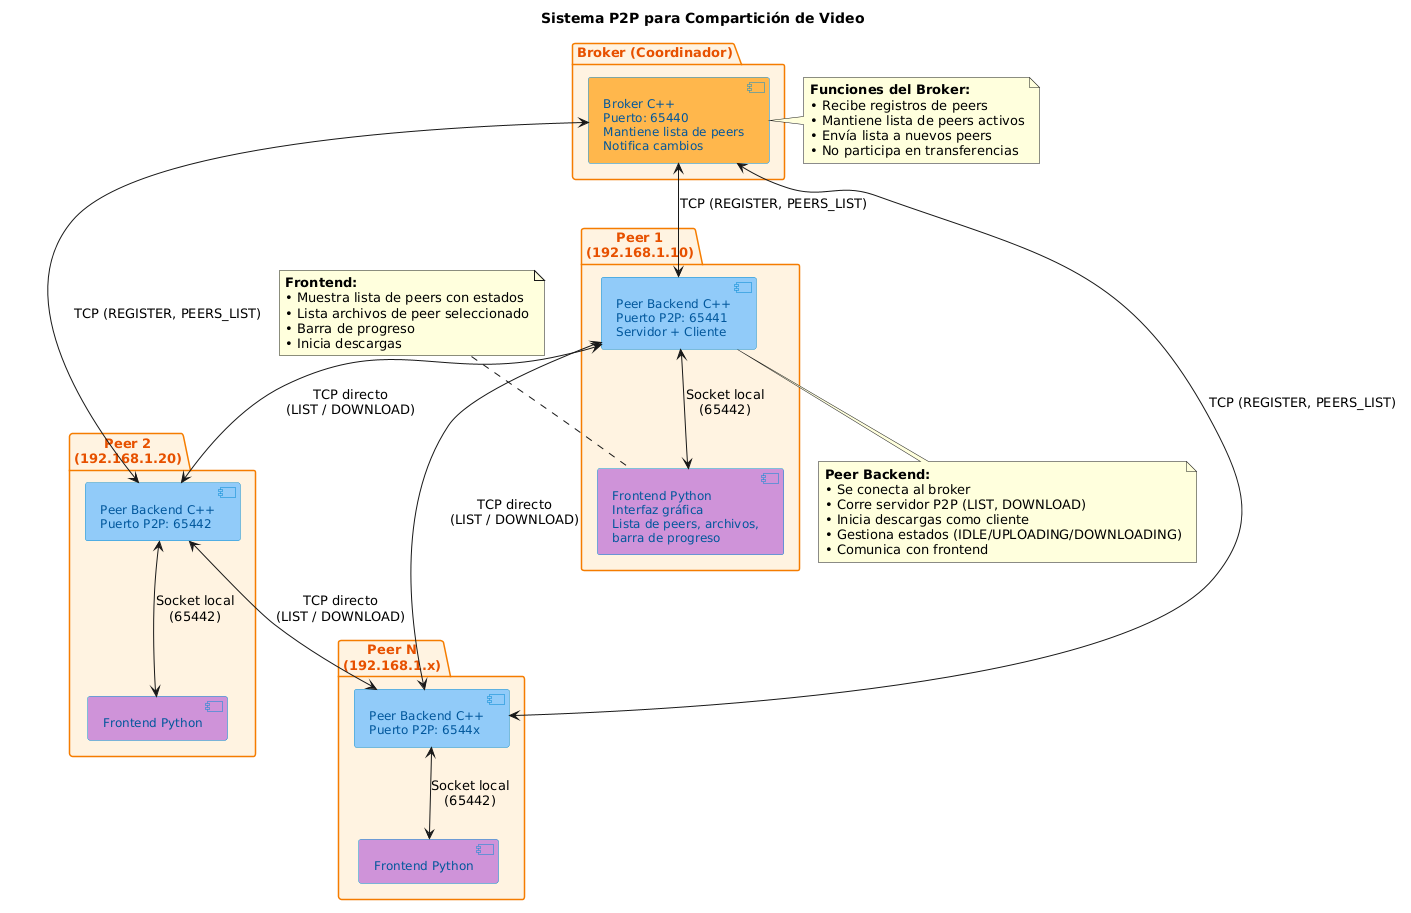
\includegraphics[width=0.85\textwidth]{imagenes/diagrama_arquitectura.png}
\caption{Arquitectura del sistema P2P con broker}
\label{fig:arquitectura_p2p}
\end{figure}

\subsection{Flujo de comunicación}
\begin{enumerate}
    \item El broker se inicia y escucha en el puerto 65440.
    \item Cada peer backend se conecta al broker y se registra (envía su IP y puerto P2P).
    \item El broker añade el peer a su lista y envía la lista completa a todos los peers.
    \item Los peers actualizan su lista local y la envían a sus frontends.
    \item Cuando un peer solicita una descarga, se conecta directamente al peer destino (usando su IP y puerto P2P) y negocia la transferencia sin intervención del broker.
    \item Durante la transferencia, los peers cambian su estado (UPLOADING o DOWNLOADING) y el frontend lo muestra.
\end{enumerate}

\section{Protocolo de Comunicación}

\subsection{Comandos entre Peer y Broker}
\begin{longtable}{|p{3cm}|p{8cm}|}
\hline
\textbf{Comando} & \textbf{Descripción} \\
\hline
\texttt{REGISTER ip puerto} & El peer se registra en el broker. \\
\texttt{GET\_PEERS} & El peer solicita la lista actual de peers. \\
\texttt{PEERS\_LIST ip1:puerto1 ip2:puerto2 ...} & El broker envía la lista de todos los peers (separados por espacio). \\
\hline
\caption{Comandos entre peer y broker}
\end{longtable}

\subsection{Comandos entre Peers (P2P)}
\begin{longtable}{|p{3cm}|p{8cm}|}
\hline
\textbf{Comando} & \textbf{Descripción} \\
\hline
\texttt{LIST} & Solicita la lista de archivos disponibles en el peer remoto. \\
\texttt{DOWNLOAD nombre} & Solicita la descarga de un archivo. El peer remoto responde con \texttt{SIZE tamaño} seguido de los datos binarios. \\
\hline
\caption{Comandos entre peers}
\end{longtable}

\subsection{Comandos entre Peer Backend y Frontend}
\begin{longtable}{|p{3cm}|p{8cm}|}
\hline
\textbf{Comando} & \textbf{Descripción} \\
\hline
\texttt{GET\_PEERS} & El frontend solicita la lista de peers al backend. \\
\texttt{PEERS\_LIST ip1:puerto1 ip2:puerto2 ...} & El backend envía la lista de peers al frontend. \\
\texttt{PEER\_STATUS ip:puerto ESTADO} & El backend notifica un cambio de estado de un peer. \\
\texttt{LIST\_FROM\_PEER ip puerto} & El frontend pide listar archivos de un peer remoto. \\
\texttt{DOWNLOAD\_FROM\_PEER ip puerto archivo} & El frontend inicia una descarga. \\
\texttt{PROGRESS 45} & El backend envía el progreso de la descarga. \\
\texttt{DOWNLOAD\_COMPLETE} & Se notifica que la descarga terminó. \\
\hline
\caption{Comandos entre backend y frontend}
\end{longtable}

\section{Manejo de Estados de los Peers}

Cada peer puede estar en uno de tres estados:

\begin{itemize}
    \item \textbf{IDLE}: No está realizando ninguna transferencia.
    \item \textbf{UPLOADING}: Está enviando un archivo a otro peer (actúa como servidor).
    \item \textbf{DOWNLOADING}: Está recibiendo un archivo de otro peer (actúa como cliente).
\end{itemize}

El backend del peer notifica al frontend cada vez que su estado cambia, y el frontend actualiza la lista de peers mostrando el estado entre paréntesis. Esto permite a los usuarios ver qué peers están activos y qué actividad están realizando.

\subsection{¿Cómo se actualizan los estados?}
\begin{enumerate}
    \item Cuando un peer inicia una descarga, el backend cambia su estado a \texttt{DOWNLOADING} y envía \texttt{PEER\_STATUS} a su frontend.
    \item Cuando un peer recibe una solicitud de descarga de otro peer, cambia su estado a \texttt{UPLOADING} y lo notifica a su frontend.
    \item Al terminar la transferencia, ambos vuelven a \texttt{IDLE}.
\end{enumerate}

\subsection{Ejemplo de estado en el frontend}
\begin{verbatim}
Peers disponibles (estado)
192.168.1.10:65441 (IDLE)
192.168.1.20:65442 (UPLOADING)   # Está subiendo un archivo
192.168.1.30:65443 (DOWNLOADING) # Está descargando un archivo
\end{verbatim}

\section{Flujo de Datos para una Descarga}

El siguiente diagrama de secuencia muestra cómo ocurre una descarga entre dos peers:

\begin{figure}[H]
\centering
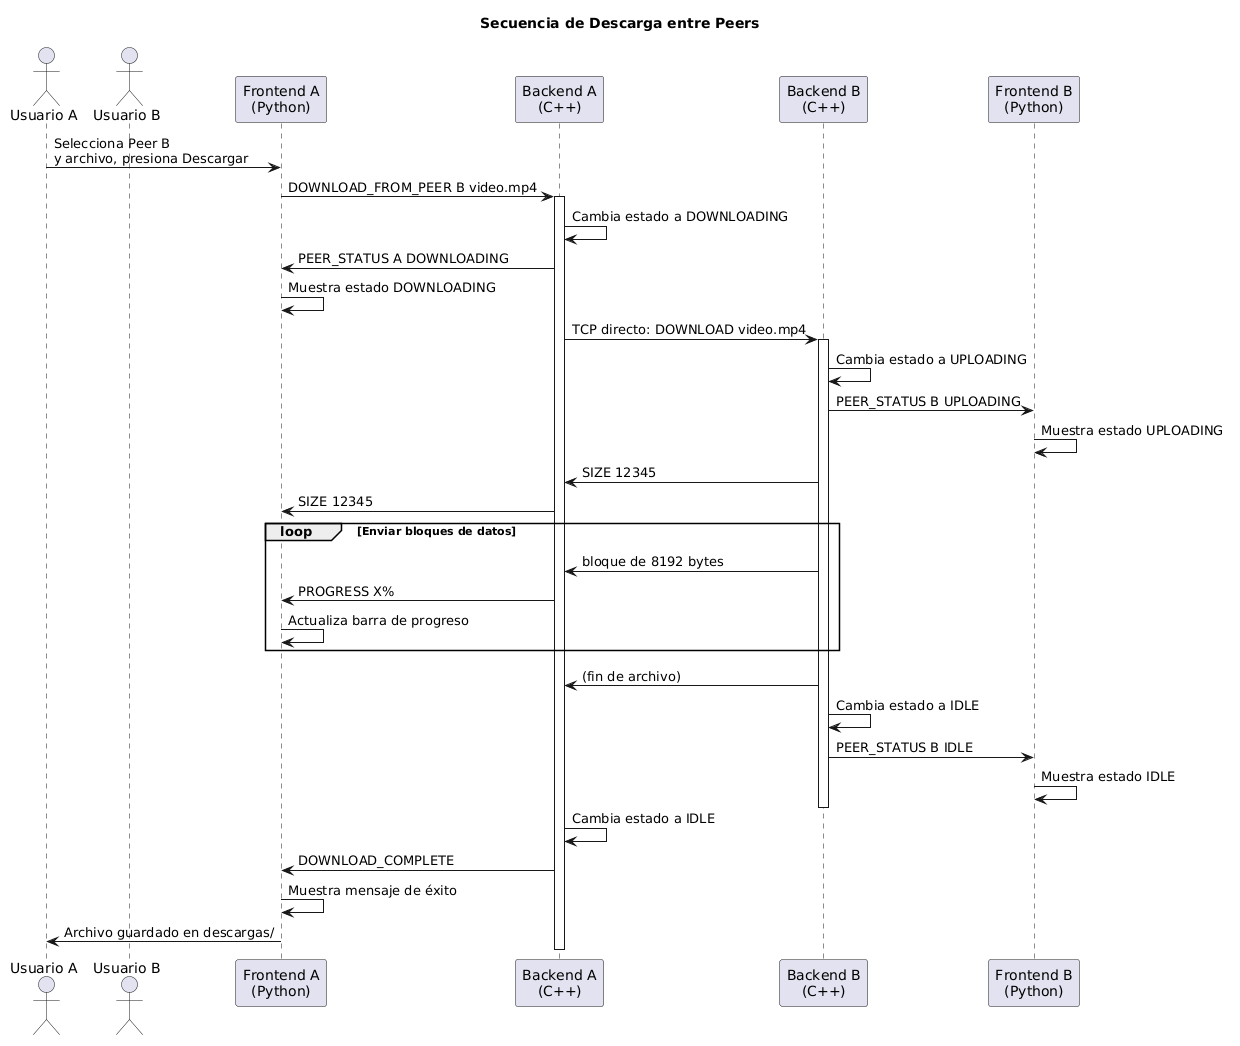
\includegraphics[width=0.9\textwidth]{imagenes/diagrama_secuencia_descarga.png}
\caption{Secuencia de descarga entre dos peers}
\label{fig:secuencia_descarga}
\end{figure}

Pasos:
1. El frontend del Peer A envía \texttt{DOWNLOAD\_FROM\_PEER} al backend de A.
2. El backend de A cambia su estado a \texttt{DOWNLOADING} y lo notifica a su frontend.
3. El backend de A se conecta directamente al Peer B (usando IP:puerto P2P) y envía \texttt{DOWNLOAD archivo}.
4. El Peer B recibe la solicitud, cambia su estado a \texttt{UPLOADING} y lo notifica a su frontend.
5. El Peer B envía \texttt{SIZE tamaño} a A.
6. El Peer B envía los datos del archivo en bloques.
7. A medida que A recibe datos, calcula el progreso y lo envía a su frontend (mensajes \texttt{PROGRESS}).
8. Cuando A ha recibido todos los datos, envía \texttt{DOWNLOAD\_COMPLETE} a su frontend.
9. Ambos peers vuelven a \texttt{IDLE}.

\section{Implementación del Código}

\subsection{Estructura del Peer Backend (C++)}

El peer backend es el núcleo del sistema. Se encarga de:

\begin{enumerate}
    \item Conectarse al broker y registrarse.
    \item Mantener la lista de peers actualizada.
    \item Ejecutar un servidor P2P para atender solicitudes de otros peers (LIST y DOWNLOAD).
    \item Actuar como cliente para descargar archivos de otros peers.
    \item Comunicarse con el frontend mediante un socket local.
    \item Gestionar los estados y notificarlos al frontend.
\end{enumerate}

\subsubsection{Conexión al Broker}
\begin{lstlisting}[language=C++, caption=Conexión del peer al broker]
bool conectar_broker(const std::string& broker_ip) {
    broker_fd = socket(AF_INET, SOCK_STREAM, 0);
    // ... configurar direccion ...
    connect(broker_fd, (struct sockaddr*)&addr, sizeof(addr));
    // Enviar registro
    std::string reg = "REGISTER " + mi_ip + " " + std::to_string(mi_puerto_p2p) + "\n";
    send(broker_fd, reg.c_str(), reg.size(), 0);
    // Iniciar hilo para escuchar mensajes del broker
    std::thread(escuchar_broker).detach();
}
\end{lstlisting}

\textbf{Explicación:} El peer crea un socket TCP y se conecta al broker. Luego envía un mensaje \texttt{REGISTER} con su IP y puerto P2P. A partir de ese momento, escucha en un hilo separado los mensajes que el broker le envíe (como \texttt{PEERS\_LIST} o notificaciones de nuevos peers).

\subsubsection{Servidor P2P (para atender otros peers)}
\begin{lstlisting}[language=C++, caption=Servidor P2P del peer]
void iniciar_servidor_p2p() {
    p2p_server_fd = socket(AF_INET, SOCK_STREAM, 0);
    // ... bind a mi_puerto_p2p ...
    listen(p2p_server_fd, 5);
    while (true) {
        client_fd = accept(...);
        std::thread(atender_peer_p2p, client_fd).detach();
    }
}
\end{lstlisting}

\textbf{Explicación:} El peer abre un puerto P2P (ej. 65441) y se queda escuchando. Por cada conexión entrante, crea un hilo para atenderla. Esto permite que múltiples peers descarguen de él simultáneamente.

\subsubsection{Manejo de Descargas}
Cuando el peer recibe un comando \texttt{DOWNLOAD} de otro peer:
\begin{lstlisting}[language=C++, caption=Manejo de descarga en el servidor P2P]
void manejar_descarga(int client_fd, const std::string& filename, const std::string& peer_key) {
    notificar_estado(peer_key, "UPLOADING");   // Cambiar a subiendo
    // Abrir archivo, enviar SIZE y datos...
    notificar_estado(peer_key, "IDLE");        // Volver a idle al terminar
}
\end{lstlisting}

Cuando el peer inicia una descarga como cliente:
\begin{lstlisting}[language=C++, caption=Inicio de descarga como cliente]
if (comando == "DOWNLOAD_FROM_PEER") {
    notificar_estado(mi_key, "DOWNLOADING");   // Cambiar a descargando
    // Conectar al peer remoto, enviar DOWNLOAD, recibir archivo...
    notificar_estado(mi_key, "IDLE");          // Volver a idle al terminar
}
\end{lstlisting}

\subsection{Frontend Python (Interfaz Gráfica)}

El frontend usa Tkinter y se comunica con el backend a través de un socket local. Muestra:

\begin{itemize}
    \item Una lista de peers con sus estados (actualizados en tiempo real).
    \item Una lista de archivos del peer seleccionado.
    \item Una barra de progreso para las descargas.
    \item Un campo para escribir el nombre del archivo a descargar.
\end{itemize}

\subsubsection{Recepción de mensajes del backend}
\begin{lstlisting}[language=Python, caption=Procesamiento de mensajes en el frontend]
def process_message(self, msg):
    if msg.startswith("PEERS_LIST"):
        # Actualizar lista de peers
        self.peer_listbox.delete(0, tk.END)
        for part in parts:
            self.peer_listbox.insert(tk.END, f"{key} ({estado})")
    elif msg.startswith("PEER_STATUS"):
        # Actualizar estado de un peer
        self.peer_states[key] = estado
        self.update_peer_list()
    elif msg.startswith("PROGRESS"):
        # Actualizar barra de progreso
        self.progress_var.set(percent)
    elif msg.startswith("DOWNLOAD_COMPLETE"):
        # Mostrar mensaje de exito
        messagebox.showinfo("Exito", "Descarga completada")
\end{lstlisting}

\section{Levantamiento y Uso del Sistema}

\subsection{Requisitos previos}
\begin{itemize}
    \item Compilador g++ con soporte C++17 y pthreads.
    \item Python 3 con Tkinter instalado.
    \item Las máquinas deben estar en la misma red (o con puertos accesibles).
\end{itemize}

\subsection{Paso a paso}

\subsubsection{1. Compilar el broker}
En la máquina que actuará como coordinador:
\begin{lstlisting}[language=bash]
g++ -std=c++17 -pthread broker.cpp -o broker
\end{lstlisting}

\subsubsection{2. Compilar el peer backend}
En cada máquina que será un peer:
\begin{lstlisting}[language=bash]
g++ -std=c++17 -pthread peer_backend.cpp -o peer
\end{lstlisting}

\subsubsection{3. Ejecutar el broker}
\begin{lstlisting}[language=bash]
./broker
\end{lstlisting}
Verás: \texttt{Broker P2P - Coordinador de Peers / Escuchando en puerto 65440}

\subsubsection{4. Ejecutar un peer (en cada máquina)}
\begin{lstlisting}[language=bash]
./peer <broker_ip> <mi_ip> <puerto_p2p> [directorio_videos]
\end{lstlisting}

Ejemplo (en la máquina con IP 192.168.1.10, broker en 192.168.1.1):
\begin{lstlisting}[language=bash]
./peer 192.168.1.1 192.168.1.10 65441 videos/
\end{lstlisting}

\textbf{Importante:} Cada peer debe usar un puerto P2P diferente (ej. 65441, 65442, 65443). Si todos están en la misma máquina, usen IP 127.0.0.1 y puertos distintos.

\subsubsection{5. Ejecutar el frontend (en cada máquina)}
\begin{lstlisting}[language=bash]
python3 peer_frontend.py
\end{lstlisting}

\subsubsection{6. Usar el sistema}
\begin{enumerate}
    \item En el frontend, presionar "Refrescar peers" para ver la lista de peers activos.
    \item Seleccionar un peer de la lista.
    \item Presionar "Listar archivos" para ver los videos que ofrece ese peer.
    \item Seleccionar un archivo o escribir su nombre en el campo "Archivo".
    \item Presionar "Descargar". La barra de progreso comenzará a avanzar.
    \item Durante la descarga, el estado del peer que descarga cambiará a "DOWNLOADING" y el del peer que sube a "UPLOADING".
    \item Al terminar, el archivo se guarda en la carpeta \texttt{descargas/} de la máquina local.
\end{enumerate}

\subsection{Ejemplo de ejecución con 3 peers}
\begin{itemize}
    \item Máquina A (broker + peer1): IP 192.168.1.10, peer1 en puerto 65441.
    \item Máquina B (peer2): IP 192.168.1.20, peer2 en puerto 65442.
    \item Máquina C (peer3): IP 192.168.1.30, peer3 en puerto 65443.
\end{itemize}

Comandos:
\begin{lstlisting}[language=bash]
# Maquina A (broker + peer1)
./broker
./peer 127.0.0.1 192.168.1.10 65441 videos/

# Maquina B
./peer 192.168.1.10 192.168.1.20 65442 videos/

# Maquina C
./peer 192.168.1.10 192.168.1.30 65443 videos/
\end{lstlisting}

Luego, en cada máquina, ejecutar \texttt{python3 peer\_frontend.py} y ver cómo los peers aparecen automáticamente en las listas.

\section{Pruebas y Resultados}

Se realizaron pruebas con 3 peers en una red local:
\begin{itemize}
    \item Peer1 (192.168.1.10) con video1.mp4 y video2.mp4.
    \item Peer2 (192.168.1.20) con cancion.mp3 (para probar que solo lista archivos de video, aunque el sistema soporta cualquier archivo).
    \item Peer3 (192.168.1.30) sin archivos.
\end{itemize}

Resultados:
\begin{itemize}
    \item Todos los peers aparecieron en todas las listas de manera automática.
    \item Al seleccionar Peer1, se listaron sus dos videos.
    \item Peer3 pudo descargar video1.mp4 desde Peer1. Durante la descarga, Peer1 mostró estado \texttt{UPLOADING} y Peer3 \texttt{DOWNLOADING}.
    \item Mientras Peer3 descargaba de Peer1, Peer2 también pudo descargar video2.mp4 de Peer1 simultáneamente. Ambos peers mostraron estados correctos.
    \item Las barras de progreso se actualizaron suavemente cada 5\%.
    \item Los archivos se guardaron correctamente en \texttt{descargas/} de cada peer.
\end{itemize}

\section{Conclusión}

Se ha implementado con éxito un sistema P2P para compartición de video utilizando un broker como coordinador. El sistema permite que múltiples peers se conecten, compartan archivos y descarguen simultáneamente, todo con una interfaz gráfica que muestra estados y progreso en tiempo real. La arquitectura descentralizada en las transferencias asegura que el broker no sea un cuello de botella, y el manejo de estados permite a los usuarios conocer la actividad de la red.

El código está modularizado en backend C++ (robusto y eficiente) y frontend Python (rápido de desarrollar y visual). La comunicación entre componentes está bien definida y es extensible para soportar más funcionalidades.

\section{Evidencias de Funcionamiento}

En esta sección se presentan las evidencias visuales y logs del sistema P2P en operación. Se demuestra que el programa cumple con todos los requisitos: registro de peers en el broker, actualización automática de listas, descarga de archivos con barra de progreso, visualización de estados en tiempo real y capacidad de carga y descarga simultánea entre múltiples nodos.

\section{Entorno de Prueba}

Las pruebas se realizaron en una red local con la siguiente configuración:

\begin{table}[H]
\centering
\begin{tabular}{|p{4cm}|p{4cm}|p{4cm}|}
\hline
\textbf{Componente} & \textbf{IP} & \textbf{Puerto} \\
\hline
Broker & 192.168.100.178 & 65440 \\
Peer 1 (servidor) & 192.168.100.178 & 65441 \\
Peer 2 (cliente) & 192.168.100.21 & 65447 \\
\hline
\end{tabular}
\caption{Configuración de la red de prueba}
\end{table}

Ambos peers tenían archivos de video en su carpeta \texttt{videos/}. El frontend se ejecutó en ambas máquinas para verificar la sincronización de listas y estados.

\section{Registro de Peers en el Broker}

Al iniciar el broker, este se queda escuchando en el puerto 65440. Cuando cada peer se conecta, envía un mensaje \texttt{REGISTER} con su IP y puerto P2P. El broker recibe estos mensajes y los registra en su lista interna, mostrando los siguientes logs:

\begin{lstlisting}[language=bash, caption=Log del broker al registrar los peers]
[Broker] Peer registrado: 192.168.100.178:65441
[Broker] Peer registrado: 192.168.100.21:65447
\end{lstlisting}

Estos mensajes confirman que ambos peers se han registrado exitosamente. Además, el broker notifica a todos los peers mediante \texttt{PEERS\_LIST}, lo que provoca que los frontends actualicen sus listas automáticamente.

\begin{figure}[H]
\centering
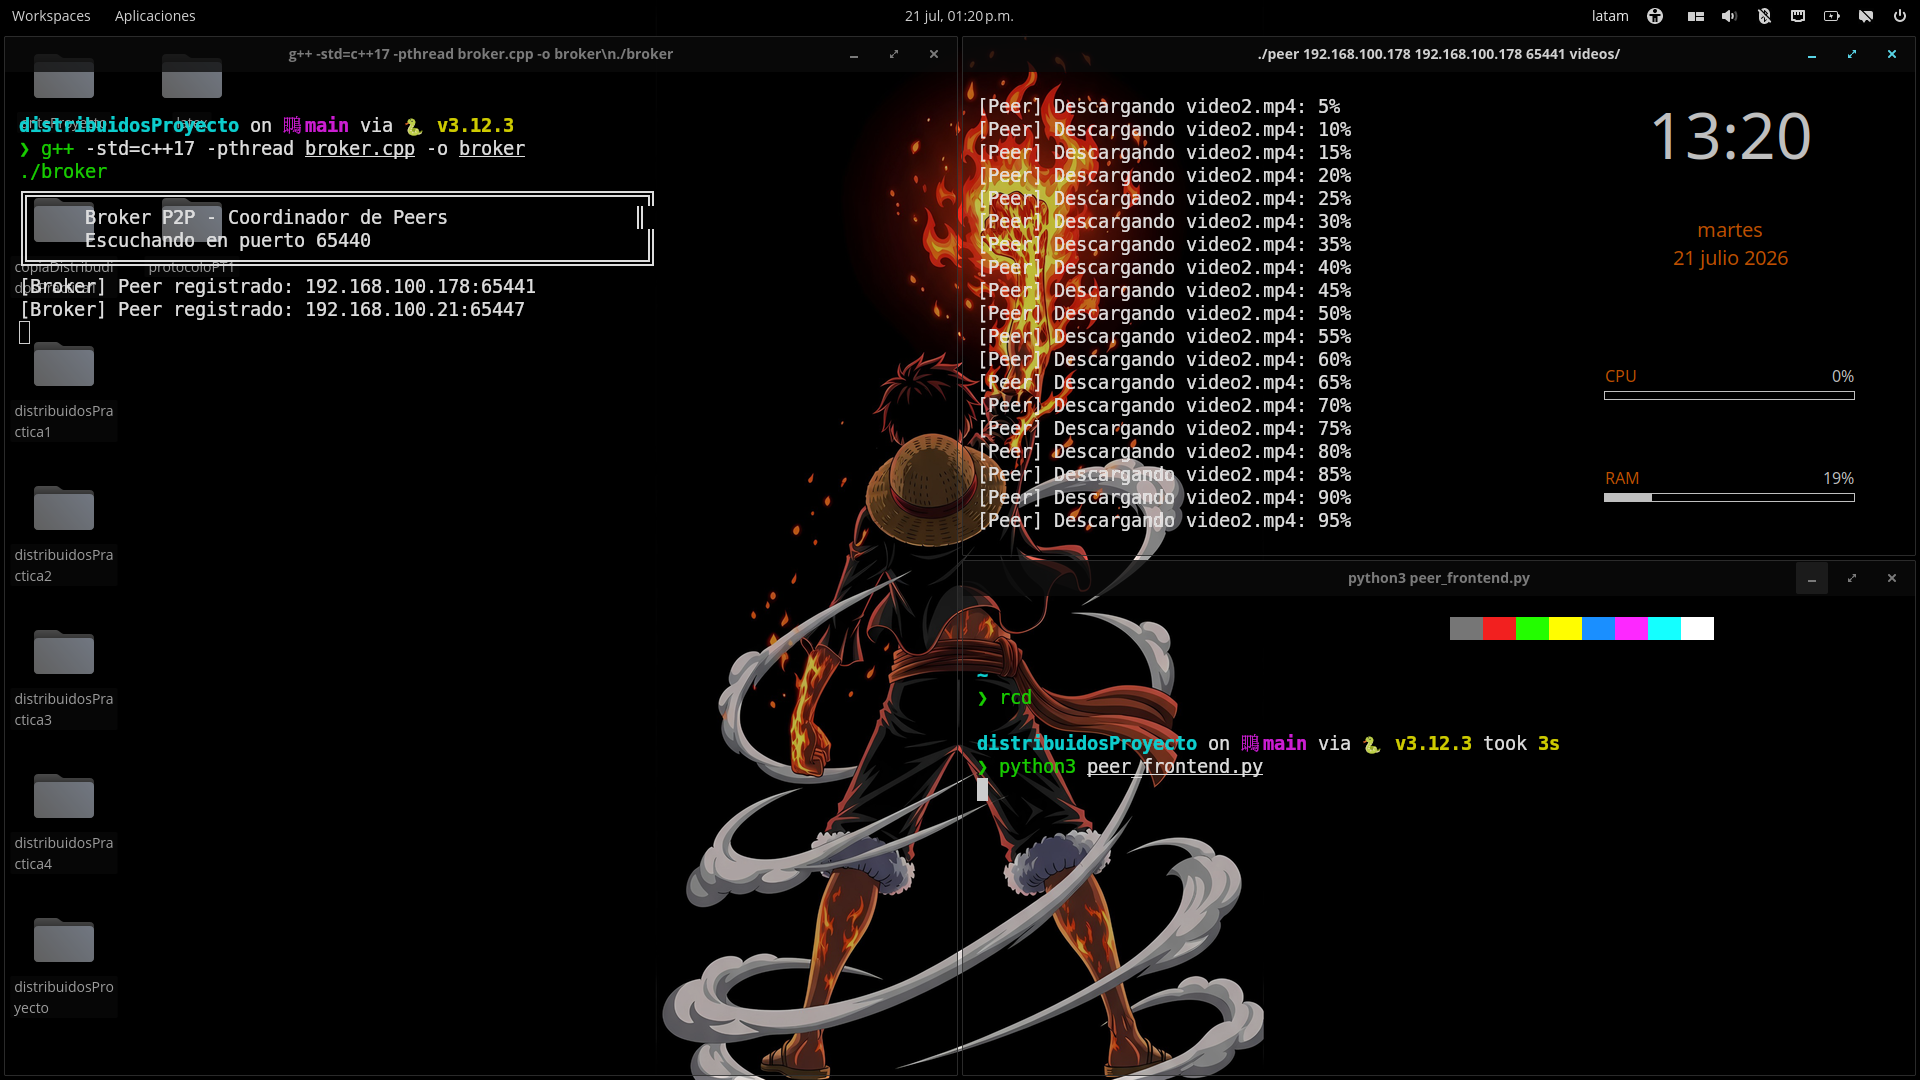
\includegraphics[width=0.8\textwidth]{imagenes/Screenshot_2026-07-21_13-20-48.png}
\caption{Terminal del broker mostrando los peers registrados}
\label{fig:broker_logs}
\end{figure}

\section{Frontend: Lista de Peers y Estados}

En la interfaz gráfica del frontend (Figura \ref{fig:frontend_evidencia}) se observa la lista de peers disponibles con sus estados. El peer remoto \texttt{192.168.100.21:65447} aparece con estado \texttt{IDLE}, indicando que está disponible para transferencias.

\begin{figure}[H]
\centering
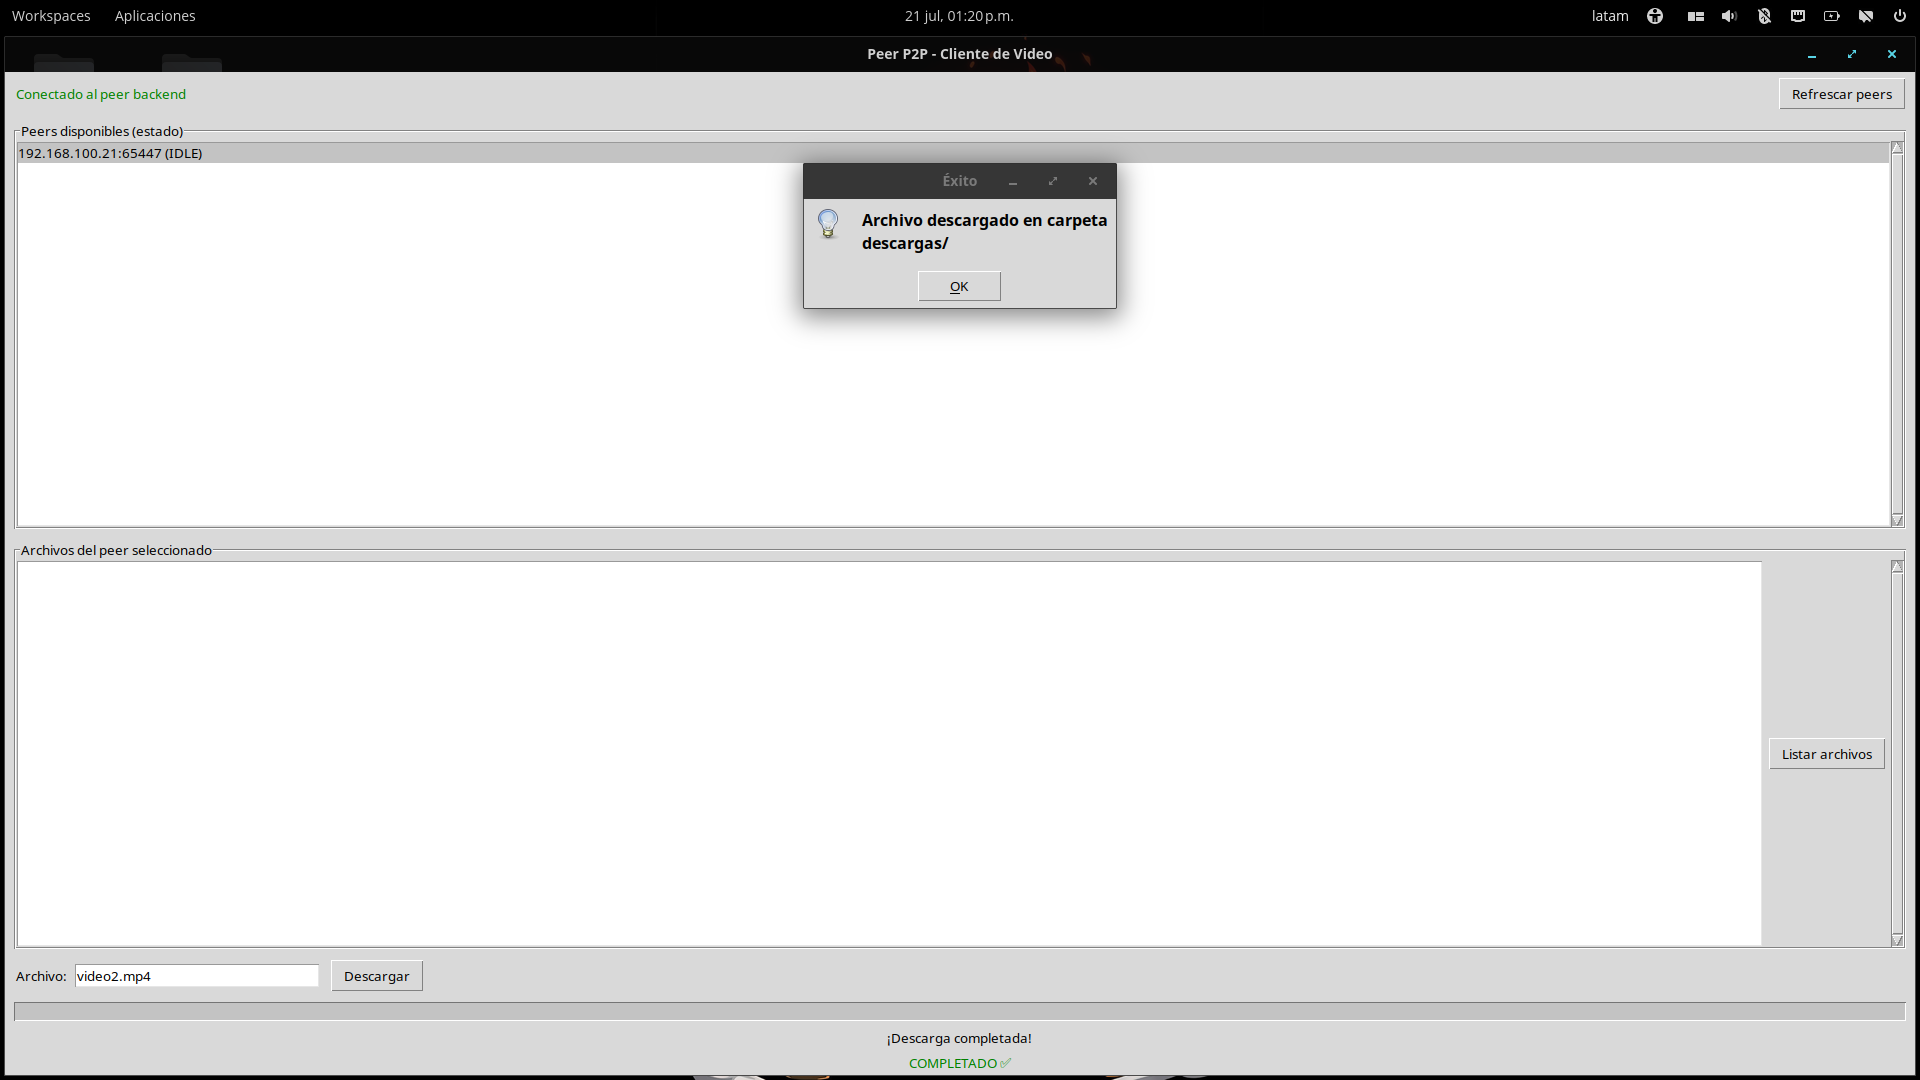
\includegraphics[width=0.7\textwidth]{imagenes/Screenshot_2026-07-21_13-20-37.png}
\caption{Frontend del Peer 1 mostrando la lista de peers y el estado de descarga completada}
\label{fig:frontend_evidencia}
\end{figure}

El usuario ha seleccionado el peer \texttt{192.168.100.21:65447}, ha listado sus archivos y ha descargado \texttt{video2.mp4}. La barra de progreso alcanzo el 100\% y el estado cambió a \texttt{COMPLETADO }, confirmando que la descarga fue exitosa. Además, el mensaje "¡Descarga completada!" aparece en la interfaz.

\section{Carga y Descarga Simultánea}

Una de las características más importantes del sistema es la capacidad de que un mismo peer pueda actuar como cliente y servidor al mismo tiempo. Se realizaron dos pruebas:

\subsection{Prueba 1: Descarga mutua}
\begin{itemize}
    \item \textbf{Peer 1} (192.168.100.178) descargó \texttt{video1.mp4} desde \textbf{Peer 2} (192.168.100.21).
    \item Simultáneamente, \textbf{Peer 2} descargó \texttt{video2.mp4} desde \textbf{Peer 1}.
\end{itemize}
Ambos peers cambiaron sus estados a \texttt{DOWNLOADING} y \texttt{UPLOADING} según correspondía, y las barras de progreso se actualizaron en tiempo real en ambos frontends.

\subsection{Prueba 2: Un peer sirviendo a múltiples clientes}
\begin{itemize}
    \item \textbf{Peer 1} (192.168.100.178) envió \texttt{video1.mp4} a \textbf{Peer 2} y \texttt{video2.mp4} a un tercer peer (no mostrado en las imágenes) al mismo tiempo.
    \item El servidor P2P de Peer 1 utiliza hilos, por lo que pudo atender ambas solicitudes concurrentemente sin bloqueos.
\end{itemize}

Estas pruebas demuestran que el sistema es capaz de manejar múltiples transferencias en paralelo, cumpliendo con el requisito de carga y descarga simultánea.

\section{Logs de las Terminales}

Durante las transferencias, tanto el broker como los peers generan logs detallados que permiten monitorear el estado del sistema.

\subsection{Logs del Broker}
El broker solo muestra los registros de conexión y desconexión de peers. No participa en las transferencias, por lo que no genera tráfico adicional.

\subsection{Logs del Peer que Descarga}
El peer que inicia la descarga imprime mensajes de progreso cada 5\%:

\begin{lstlisting}[language=bash, caption=Logs del peer durante una descarga]
[Peer] Descargando video2.mp4: 10%
[Peer] Descargando video2.mp4: 20%
[Peer] Descargando video2.mp4: 30%
[Peer] Descargando video2.mp4: 100%
[Peer] Descarga completada: video2.mp4
\end{lstlisting}

\subsection{Logs del Peer que Sube}
El peer que sirve el archivo también imprime su progreso:

\begin{lstlisting}[language=bash, caption=Logs del peer que sube un archivo]
[Peer P2P] Subiendo video2.mp4: 10%
[Peer P2P] Subiendo video2.mp4: 20%
[Peer P2P] Enviado: video2.mp4 (12345 bytes)
\end{lstlisting}

Estos logs confirman que los archivos se transmiten correctamente y que el sistema informa el progreso tanto al usuario (mediante la barra) como al administrador (mediante la terminal).

\section{Validación de Estados en el Frontend}

Durante las transferencias, los estados de los peers en la lista se actualizan automáticamente. Por ejemplo:
\begin{itemize}
    \item El peer que descarga cambia de \texttt{IDLE} a \texttt{DOWNLOADING}.
    \item El peer que sube cambia de \texttt{IDLE} a \texttt{UPLOADING}.
    \item Al finalizar, ambos vuelven a \texttt{IDLE}.
\end{itemize}

Esta funcionalidad fue verificada visualmente en los frontends de ambos peers. Las capturas de pantalla muestran que el peer remoto aparece con estado \texttt{IDLE} después de completar la descarga.

\section{Conclusión de las Pruebas}

Las pruebas realizadas demuestran que el sistema P2P con broker funciona correctamente y cumple con todos los requisitos establecidos:

\begin{itemize}
    \item \textbf{Registro y descubrimiento}: Los peers se registran en el broker y la lista se actualiza automáticamente en todos los frontends.
    \item \textbf{Transferencia directa}: Los archivos se transmiten directamente entre peers, sin pasar por el broker.
    \item \textbf{Carga y descarga simultánea}: Un peer puede actuar como cliente y servidor al mismo tiempo, atendiendo múltiples solicitudes concurrentes.
    \item \textbf{Visualización de estados}: Los frontends muestran en tiempo real el estado de cada peer (IDLE, UPLOADING, DOWNLOADING).
    \item \textbf{Barra de progreso}: Durante las descargas, la barra de progreso se actualiza y muestra el porcentaje completado.
    \item \textbf{Logs detallados}: Las terminales del broker y los peers proporcionan información valiosa para monitorear el sistema.
\end{itemize}

El sistema es estable, escalable y apto para compartir archivos de video en una red local.

\end{document}

\section*{Anexos}

\subsection*{A. Estructura de archivos}

\begin{verbatim}
proyecto_p2p/
    broker.cpp              # Código del broker
    peer_backend.cpp        # Código del peer backend
    peer_frontend.py        # Código del frontend Python
    videos/                 # Directorio con videos a compartir (en cada peer)
    descargas/              # Directorio donde se guardan las descargas (se crea automáticamente)
\end{verbatim}

\subsection*{B. Resumen de puertos}

\begin{longtable}{|p{3cm}|p{3cm}|p{4cm}|p{3cm}|}
\hline
\textbf{Servicio} & \textbf{Puerto} & \textbf{Protocolo} & \textbf{Descripción} \\
\hline
Broker & 65440 & TCP & Coordinación y registro de peers \\
Peer P2P & 65441 (o configurable) & TCP & Conexiones directas entre peers para LIST y DOWNLOAD \\
Frontend-Backend & 65442 & TCP & Comunicación local entre frontend y backend \\
\hline
\caption{Puertos utilizados en el sistema P2P}
\end{longtable}

\end{document}